The concept of implementation can be divided into the used packages (\emph{Stable Baselines3, Gym Pybullet Drones, ...}), the scripts, the environment classes and different support classes (\cref{fig:concept}).\\
Stable Baselines3 is used as implementation of the PPO algorithm (\cref{alg:ppo}) in order to achieve the tasks. Gym Pybullet Drones has already some environments and is the foundation of the simulation. It already provides a suitable step function and a well designed physics engine.\\
The scripts (\cref{sec:scripts} , lila) are used to either learn the agent on a given environment or evaluate it.\\
The environment classes(\cref{sec:env}, green) inherit from a \emph{Gym Environment} and models a MDP. By modelling this MDP precisely, it is defined what is learned later by the intelligent agent. It uses the wind class in order to model a harsh environment.
In addition, there are a couple of evaluation tools (\cref{sec:tools}, red), that supports the implemented classes.\\
\newline
The whole concept is implemented in Python3.x with the use of a \emph{conda environment}.

\begin{figure}[htp]
	\centering
	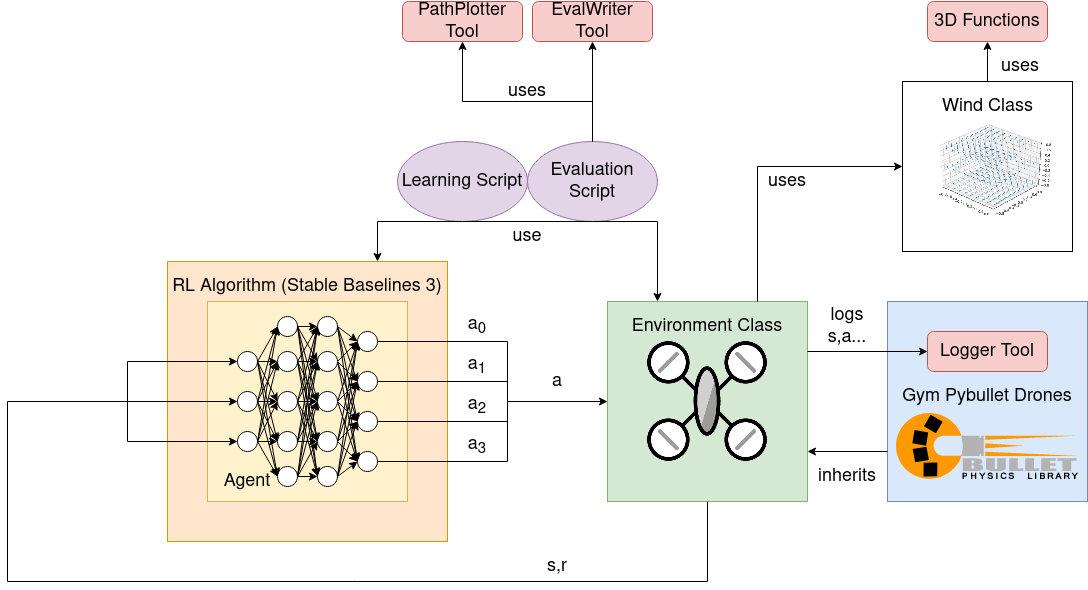
\includegraphics[width= \linewidth]{figures/concept.png}
	\caption{Concept of the implemented software: the different tools(red), scripts(violet) that are used in order to learn the intelligent Agent robust flight control with the use of RL.}
	\label{fig:concept}
\end{figure}
\newpage

\section{Environment Classes} \label{sec:env}



\subsection{WindSingleAgentAviary Environment Class}

\newpage

\subsubsection{Wind Class}
\begin{figure}
	\centering
	\begin{subfigure}{0.32\linewidth}
		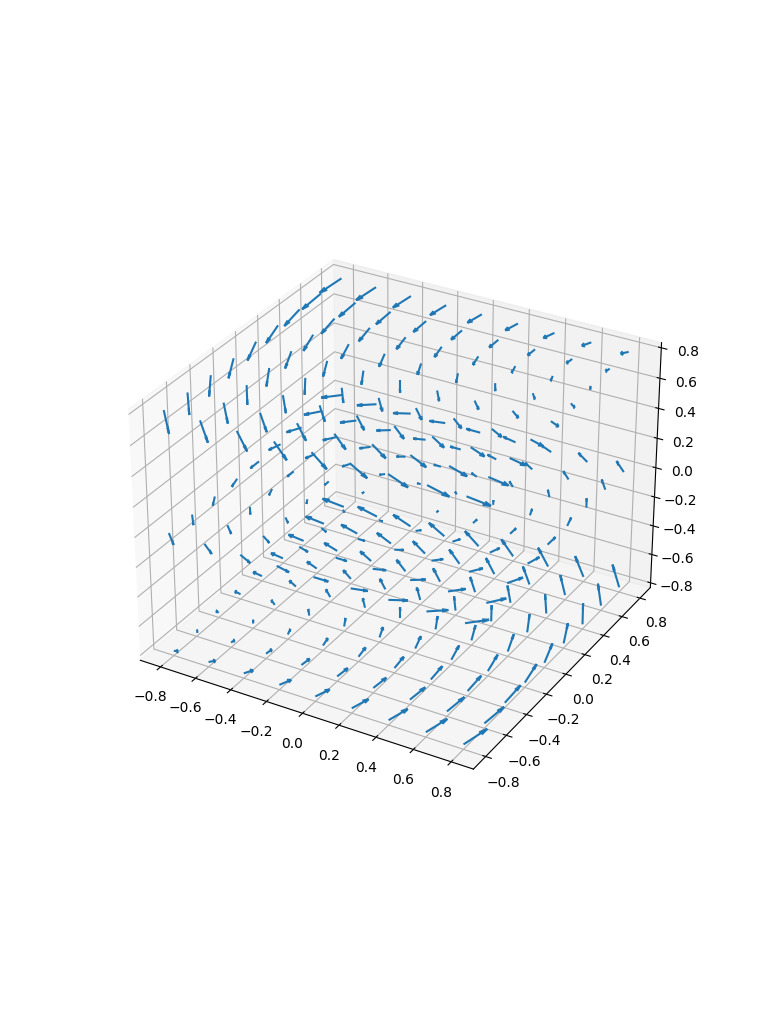
\includegraphics[width=\linewidth]{figures/wind4.png}
		\caption{}
		\label{eq:wind5}
	\end{subfigure}
	\begin{subfigure}{0.32\linewidth}
		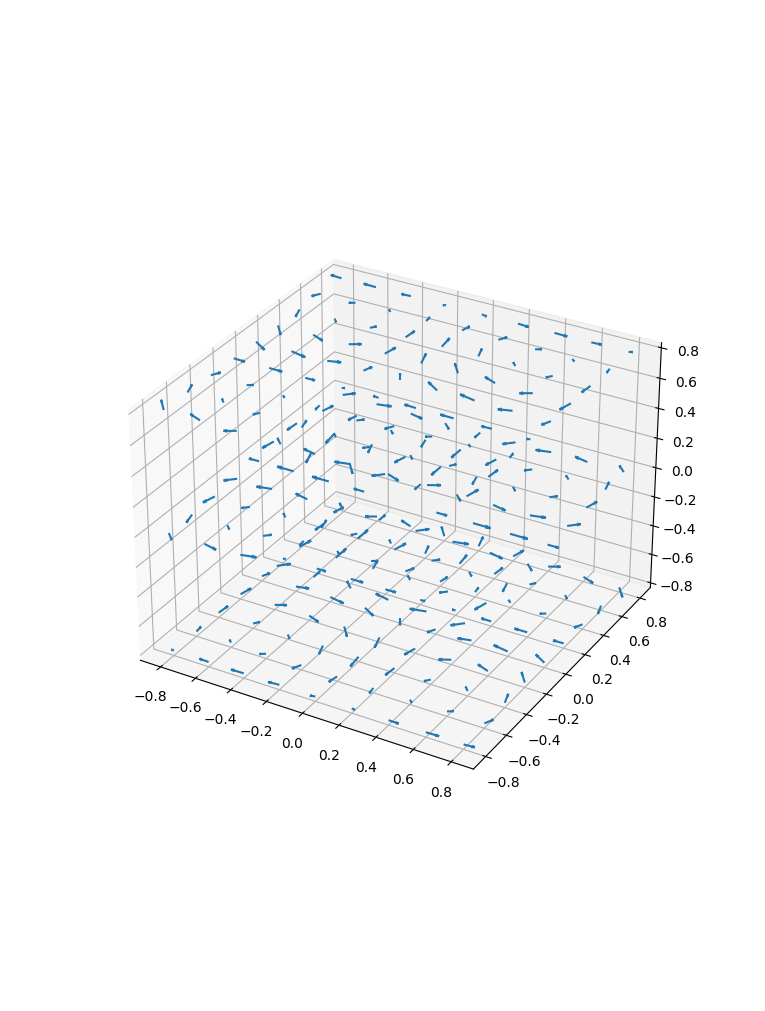
\includegraphics[width=\linewidth]{figures/wind2.png}
		\caption{}
		\label{fig:wind1}
	\end{subfigure}
	\begin{subfigure}{0.32\linewidth}
		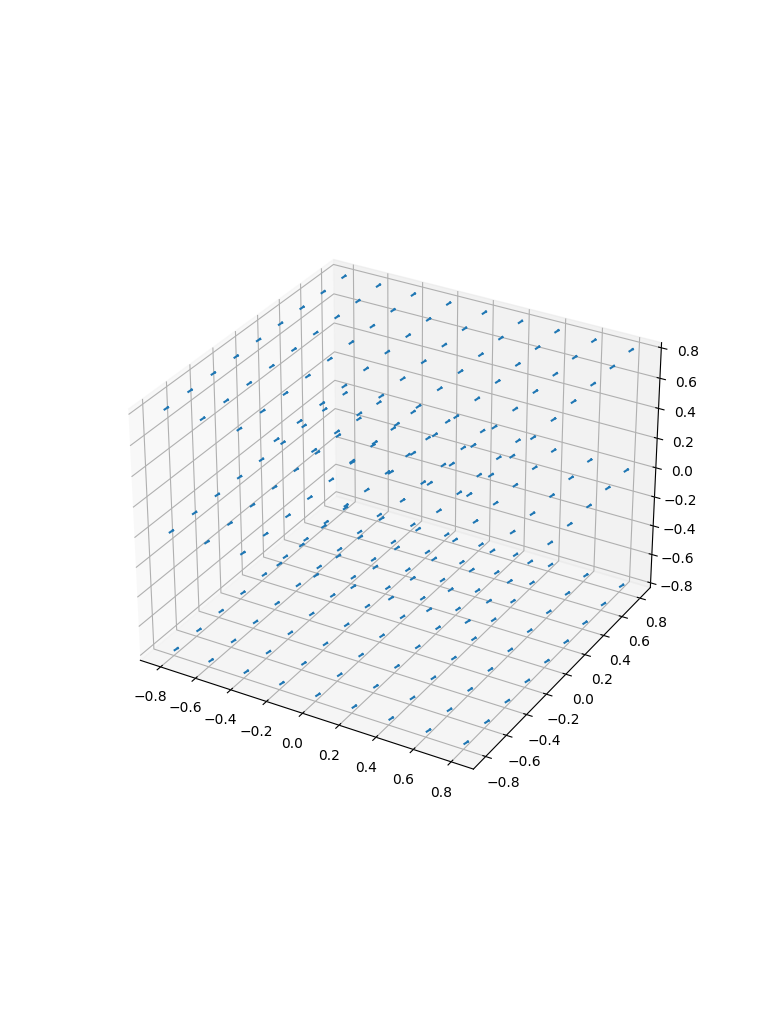
\includegraphics[width=\linewidth]{figures/wind3.png}
		\caption{}
		\label{fig:wind0}
	\end{subfigure}
	\caption{Visualization of three different wind fields. Vecotors represent a force vector that impacts the drone in the matching position. (a)  is a random vector field made with a 3D function, (b) a predefined trignometric vortex vecotr field and (c) with a random linear vector field.}
\end{figure}
The \emph{Wind Class} is an essentiell class in order to simulate a turbulent condition. Basically the class returns a 3 dimensional force vector $W$ based on the $x,y,z$ position of the drone. This force vector is then applied in the environment and pushes the drone in the matching direction. On initialization the wind is given a force bound $w [N]$ and a type. All vectors are being clipped to this amount of force in order to simulate wind fields of different strengths. In addition, the clipping method adds some guassian distributed randomness to each coordinate with the clipped vlaue as mean and a standard deviation of $0.003$. \\
\newline
\emph{Type 0} simulates a random, constant wind field that applies the same random force vector at each position (\cref{eq:wind0}). The random coordinates $r_i$ are choosen with respect to a gaussian distribution with the mean of $\frac{w}{2}$ and a standard deviation of $0.03$. As a consequence, the length of the force vector $|\overrightarrow{W}|$ is distibuted with a mean of $0.866w$. A visualization of type 0 wind field can be seen in \cref{fig:wind0}.
\begin{align} \label{eq:wind0}
	\overrightarrow{W} &= clip(\left(
	\begin{array}{c}
		r_0\\
		r_1\\
		r_2\\
	\end{array}
	\right))\\
	r_i &\sim \mathbb{N}(\frac{w}{2}, 0.03)\\
	\mathbb{E}|\overrightarrow{W}| &= \sqrt{3 \cdot \frac{w^2}{4}} \approx 0.866 w
\end{align}

\newpage

\emph{Type 1} is a trigonometric wind field with central vortex. A visualization can be seen in \cref{fig:wind1}.
\begin{align} \label{eq:wind1}
	\overrightarrow{W} = clip(\left(
	\begin{array}{c}
		\sin(\pi \cdot x) \cdot \cos(\pi \cdot y) \cdot \cos(\pi \cdot z)\\
		- \cos(\pi \cdot x) \cdot \sin(\pi \cdot y) \cdot \cos(\pi \cdot z)\\
		\sqrt{\frac{2}{3}} \cdot \cos(\pi \cdot x) \cdot \cos(
		\pi \cdot y) \cdot \sin(\pi \cdot z)\\
	\end{array}
	\right))
\end{align}
\newline

\emph{Type 2} is a wind field that is linear in each axis. Like seen in type 0 wind fields a random gaussion distributed factor $r_i$ is used that indicate how steep each of the linear functions is.
\begin{align}
	\overrightarrow{W} &= clip(\left(
	\begin{array}{c}
		r_0 \cdot x\\
		r_1 \cdot y\\
		r_2 \cdot z\\
	\end{array}
	\right))\\
	r_i &\sim \mathbb{N}(\frac{w}{2}, 0.03)
\end{align}
\newline

\emph{Type 3} simulates a basic, random wind field with a central vortex. Therefore, it uses random signs.
\begin{align}
	\overrightarrow{W} &= clip(\left(
	\begin{array}{c}
		\pm y\\
		\pm x\\
		\pm z\\
	\end{array}
	\right))
\end{align}
\newline

\emph{Type 4} is a random wind field with a central vortex, that shows a little bit more complexity.
\begin{align}
	\overrightarrow{W} &= clip(\left(
	\begin{array}{c}
		x \pm y\\
		z \pm x\\
		y \pm z\\
	\end{array}
	\right))
\end{align}
\newline

\emph{Type 5} is a completly random wind field based on three random 3D functions $f, f', f'': \mathbb{R}^3 \to \mathbb{R}$. As a conseqeunce, a lot of different, complex wind field can be created like seen in \cref{eq:wind5} that posesses different functions in each coordinate.\\

A \emph{3D function} can have a lot of different forms and should be described inductive. There are a base set of functions mapping from $\mathbb{R}^3 \to \mathbb{R}$ (\cref{eq:base}). In addition there are two rules that inductively form the whole set of functions. If $g$ already is a 3DFunction then also $\sin(g), \cos(g), 2 \cdot x \cdot \sin(g), \sqrt{g}, e^g$ are 3DFunctions (\cref{eq:rule0}). If $g$ and $h$ are 3DFunctions then $g+h$ is also a 3Dfunction (\cref{eq:rule1}). Since there could be an endless regression, the induction is closed after only one step in order to avoid a stack overflow in implementation. 

\newpage
\begin{align}
	&\textbf{Base set:} \notag \\
	&F^0 = \{0, 1, x + y + z, x + y, x + z, y + z, 
	x \cdot y \cdot z, x \cdot y, x \cdot z, y \cdot z\} \label{eq:base}\\
	&\textbf{Rules:} \notag \\
	&\forall n < 2 \quad g \in F^n \land h \in F^n \rightarrow F^{n+1} = F^n \cup \{ 
	 g + h\} \label{eq:rule0}\\
	&\forall n < 2 \quad g \in F^n \rightarrow F^{n+1} = F^n \cup \{ \sin(g), \cos(g), 2 \cdot x \cdot \sin(g), \sqrt{g}, e^g\} \label{eq:rule1}
\end{align}
\newline
If no type is specified, then the wind field is of a choosen random type.
Since type 5 is the most complex type of wind field, the others might not be really needed, because simalar wind fields like a vortex can still be approximated with the use of the 3D functions. However, it is still preferable to be able to choose a simple wind field at first before increasing complexity. In addition, there is the possibilty to evaluate agents in different wind fields.

\subsubsection{Modes}\label{sec:modes}
Since the WindSingleAgentAviary class is meant as flexible class that more complex classes can inherit from, it has different modes that influences the position of the goal and the type of the wind (\cref{tab:mode}).
The use of modes is helpful in order to debug the environment end slowly increment the complexity of the RL problem.

\begin{table}[htp]
	\centering
	\caption{The different Modes of a WindSingleAgentAviary environment.}\label{tab:mode}
	\begin{tabular}{|c|c|c|}
		\hline
		Mode & Goal & Wind\\
		\hline
		0 & $\left(\begin{array}{c}
			0\\
			0\\
			0.5\\
		\end{array}
		\right)$ & no wind\\
		\hline
		1 & $\left(\begin{array}{c}
			0\\
			0\\
			g_z\\
		\end{array}
		\right) \qquad g_z \in [0.3, 0.8]$& no wind\\
		\hline
		2 & $\left(\begin{array}{c}
			g_x\\
			g_y\\
			g_z\\
		\end{array}
		\right) \qquad g_x \in [-0.5, 0.5],\quad g_y \in [-0.5, 0.5],\quad g_z \in [0.3, 0.8]$& no wind\\
		\hline
		3 & $\left(\begin{array}{c}
			g_x\\
			g_y\\
			g_z\\
		\end{array}
		\right) \qquad g_x \in [-0.5, 0.5],\quad g_y \in [-0.5, 0.5],\quad g_z \in [0.3, 0.8]$& type 0\\
		\hline
		4 & $\left(\begin{array}{c}
			g_x\\
			g_y\\
			g_z\\
		\end{array}
		\right) \qquad g_x \in [-0.5, 0.5],\quad g_y \in [-0.5, 0.5],\quad g_z \in [0.3, 0.8]$& type 5\\
		\hline
	\end{tabular}
\end{table}

\newpage

\subsubsection{Observation Space \& State Space}
The state space $S$ defines the state vector of the drone in the environment and possesses a dimensionality of $23$. This state is only used inside the evironment and consists of the current position $x_p, y_p, z_p$ in each axis, the roll, pitch and yaw angles $\Theta_p, \phi_p, \psi_p$ as well as represented as quaterion $q$, the velocities $\dot{x_p}, \dot{y_p}, \dot{z_p}$, the angular velocities $dot{\Theta_p}, \dot{\phi_p}, \dot{\psi_p}$, the goal position $x_g, y_g, z_g$ and the last clipped action $a_t$. With the use of this drone state space the observations are calculated.\\
\newline
The observation space $\sigma$ is a subset of the state space $S$ with the dimensionality of 15. The observation space is implemented as a \emph{spaces box} of type \emph{float32} wich are mainly ranged within $[-1, 1]$ with the exception of the z coordinate of the position $z_p$ and goal $z_g$. Because there is floor defined as a plain at the height of $0$, which inherits a collision body, the drone is not able to reach a negative z coordinate. As a consequence, these are ranged to $[0,1]$.
\newline
\begin{align}
	\sigma_t &= (x_p,y_p,z_p, \Theta_p, \phi_p, \psi_p, \dot{x_p}, \dot{y_p}, \dot{z_p}, \dot{\Theta_p}, \dot{\phi_p}, \dot{\psi_p}, x_g, y_g, z_g) \label{eq:obs}
\end{align}
\newline
Each observation $\sigma_t$ consists of the current position $x_p, y_p, z_p$ in each axis, the roll, pitch and yaw angles $\Theta_p, \phi_p, \psi_p$, the velocities $\dot{x_p}, \dot{y_p}, \dot{z_p}$, the angular velocities $dot{\Theta_p}, \dot{\phi_p}, \dot{\psi_p}$ and the goal position $x_g, y_g, z_g$ (\cref{eq:obs}). These observations are given to the NN in order to approximate the optimal action $a$ that satefies the defined RL problem.\\
\newline
Like previously mentioned, all observations are ranged in order to prohibit inputs of different magnitude that could disrupt the learning process. This is done with the use of the method \emph{\_clipAndNormalizeState} which gets the current state $s_t$ and normalizes it to the defined range (\cref{eq:clipnorm}). First, it clips it to predifined values $v$ and then normalizes it by deviding with the matching predefined value $v_i, i\in[0,11]$. If wanted, a warning can be printed each time a state parameter has to be clipped. By clipping x and y to a value in $[-20,20]$ there is a predifed limit of maximal distance, in which there is a reasonable option to learn robust flight. Analogue the z component is clipped to $[-10,10]$, roll and pitch to $[-\pi, \pi]$, the translation velocities to $[-3, 3]$ in x,y and to $[-2,2]$ in z direction. 
\newline
\begin{align}
	\sigma_t \leftarrow clip(s_t) / v \label{eq:clipnorm}
\end{align}
\newline

\newpage

\subsubsection{Action Space}
The WindSingleAgentAviary Environment possesses three different type of action spaces, that are processed in different ways to the \emph{rpm (rotation per minute)} of the four motors (\cref{tab:act}). Nevertheless, all action types are continuous and are ranged in $[-1, 1]$.\\
\newline
\emph{one\_d\_rpm} is a one dimensional action space. The chosen action $a$ is processed to range of $\alpha$ about the \emph{hover\_rpm} to a 4-tupel of rpms. The hover\_rpm is defined as the rpm that corresponds to hovering (\cref{sec:hover}). The 4-tupel is then forwarded to the motors. As a consequence of this limitation, the drone can only perform hovering, rising and falling movements and can not influence its $x,y$ position or $\Theta, \phi, \psi$. Also, the translational speed $v_z$ is limited by the size of $\alpha$.\\
\newline
\emph{rpm} is a 4 dimensional action space. The actions are processed within a range of $\alpha$ about the hover\_rpm to a 4-tupel of rpms. The drone is not limited in any dimensionality, but the task increases in complexity. Due to \cref{form:quad}, \cref{form:quad2}, \cref{form:quad3}, \cref{form:quad4} even a small difference in rpms can lead to an unstable flight or even a crash, because the roll or pitch angle is to high. Also, all translational an rotational speeds are limited by the size of $\alpha$. Because of the higher complexity, it is expected, that the training takes noticeable more time.\\
\newline
\emph{vel} is a top level, 4-dimensional action space. The action consists of a velocity vector $v = (a_0, a_1, a_2)$ and its size $a_3$.  Since it is a top level action space, the actions are not corresponding directly to the rpms, but a pid controller (\cref{sec:pid}) is used in order to control the rpms. The basic pid controller is part of Gym Pybullet Drones \cite{panerati2021learning} and must be tuned for the used quadrocopter. It mainly receives the state $S$ of the drone, as well as the targeted velocity, which is calculated with the use of the actions. Therefore, $a_3$ is multiplicated with speed limit of the drone in order to derange the action. Also, the velocity vector $v$ is normalized to a length of $1$.\\
The drone is not limited in any dimensionality and the task is less complex then setting rpm directly. Stability of the flight is now mainly controlled by the pid controller, so it is bounded by the typical pid constraints in harsh environments and not adaptable.
\begin{table}
	\centering
	\caption{The different ActionTypes with the corresponding dimensionality of the action, its range and how it is processed.}\label{tab:act}
	\begin{tabular}{c|c|c|c}
		ActionType & dim & range & processing\\
		\hline
		\emph{one\_d\_rpm} & $|a| = 1$ & $a_i \in [-1, 1]$ & $rpm = (hover\_rpm \cdot (1 + \alpha \cdot  a)) \cdot (1, 1, 1, 1)$ \\
		\emph{rpm} & $|a| = 4$ & $a_i \in [-1, 1]$ & $rpm =  hover\_rpm \cdot (1 + \alpha \cdot  a)$ \\
		\emph{vel} & $|a| = 4$ & $a_i \in [-1,1]$ & $rpm = pid(S, vel= limit \cdot  |a_3| \cdot \frac{(a_0,a_1,a_2)}{|(a_0,a_1,a_2)|})$
	\end{tabular}
\end{table}


\newpage

\subsubsection{Reward}
\begin{figure}
	\centering
	\begin{subfigure}{0.3\linewidth}
		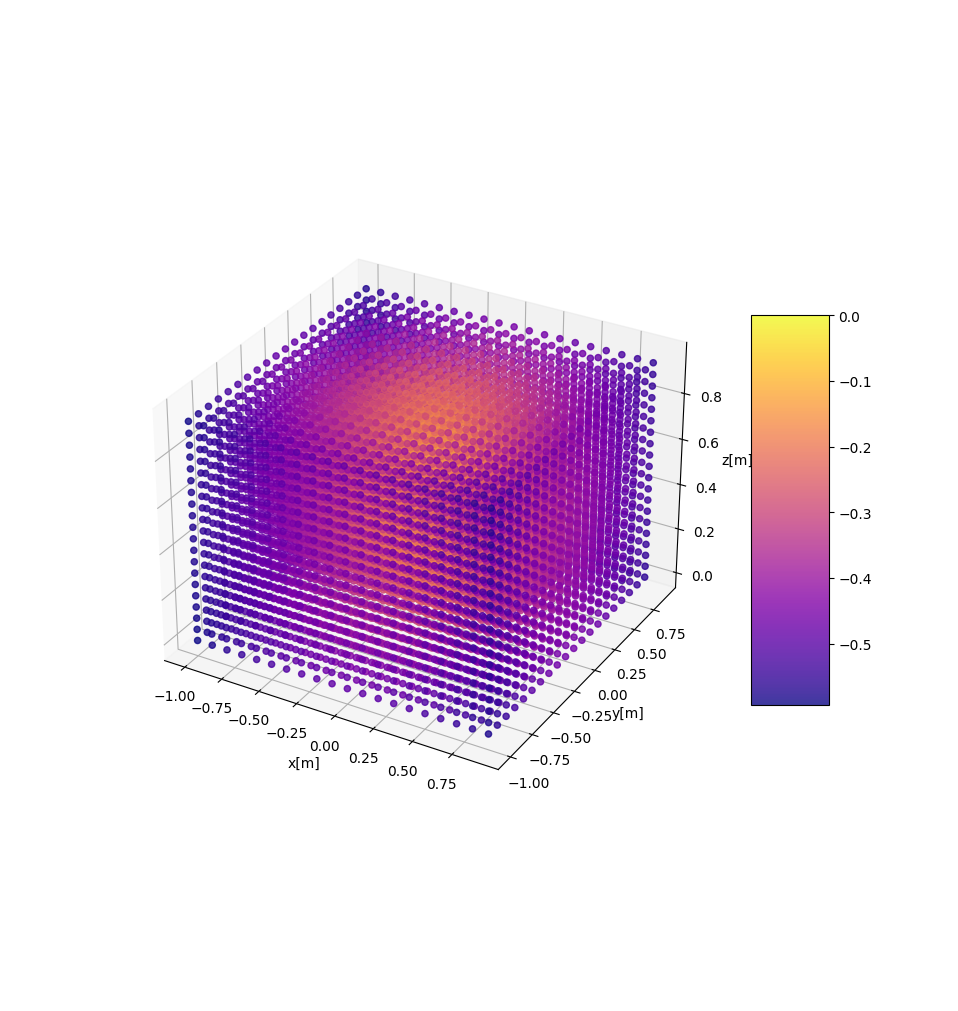
\includegraphics[width=\linewidth]{figures/rew3d.png}
		\caption{}
	\end{subfigure}
	\begin{subfigure}{0.3\linewidth}
		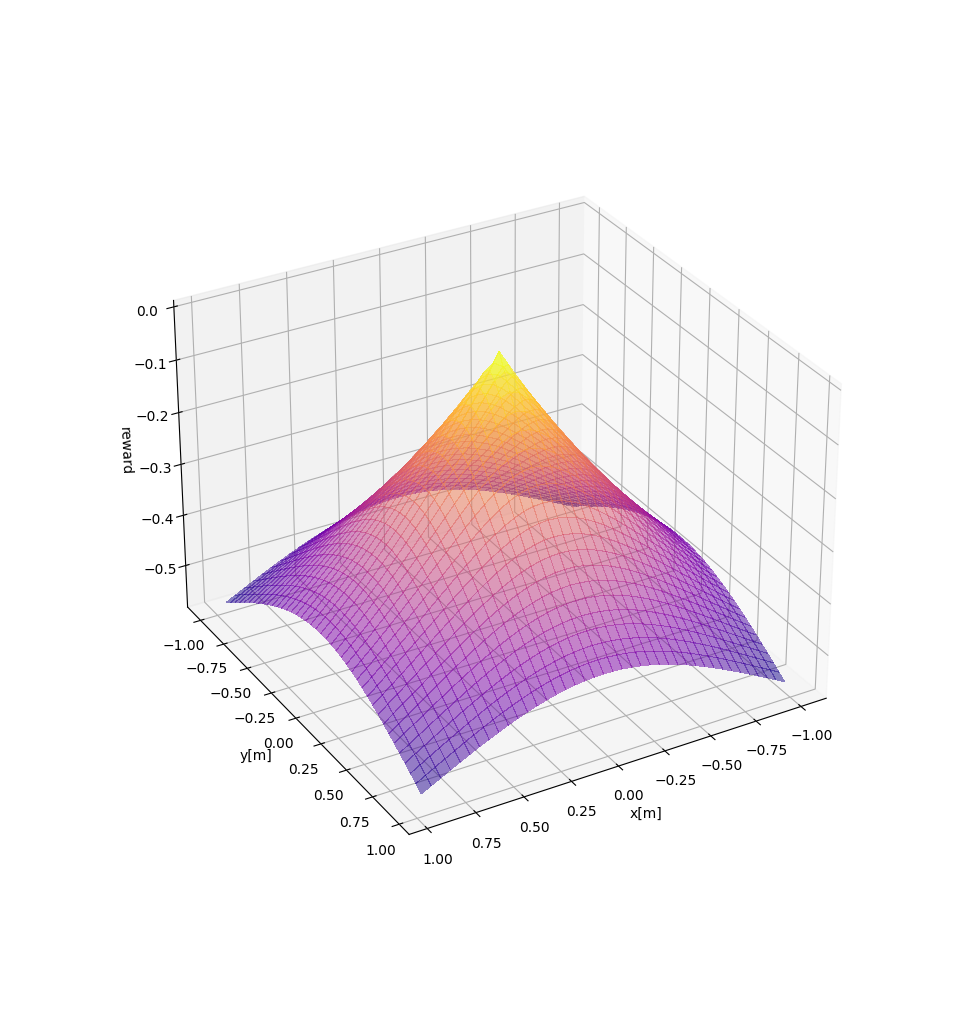
\includegraphics[width=\linewidth]{figures/rewXY.png}
		\caption{}
	\end{subfigure}
	\begin{subfigure}{0.3\linewidth}
		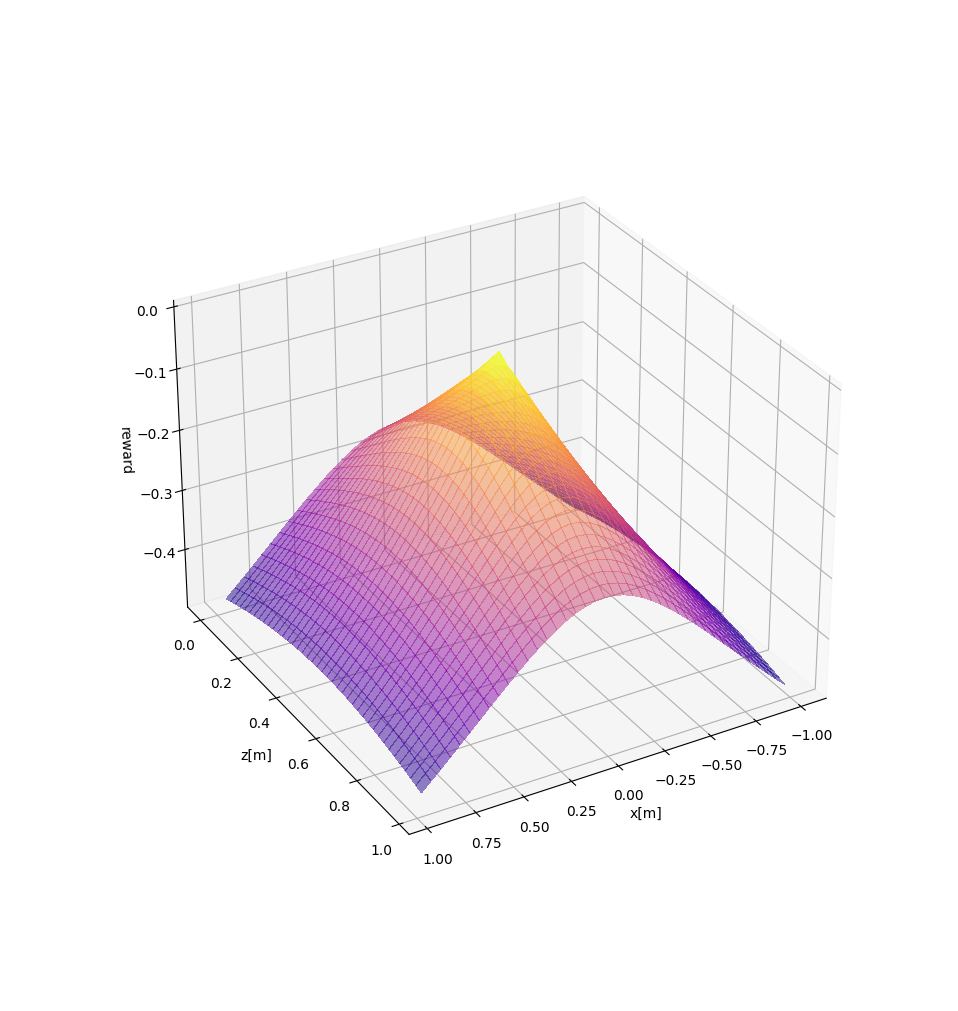
\includegraphics[width=\linewidth]{figures/rewXZ.png}
		\caption{}
	\end{subfigure}
	\caption{Visualization of the used reward function with the goal ($0,0,0.5$) and a colour scale for different positions in space.}
\end{figure}

\begin{align}
	r_t = e^{-0.6 \cdot |dist_t|} - 1 &= e^{-0.6 \cdot |goal - pos_t|} - 1 \label{eq:rew}\\
	\lim_{dist_t \to \infty} r_t &= -1\\
	\lim_{dist_t \to 0+} r_t &= 0
\end{align}

\newpage

\begin{figure}
	\centering
	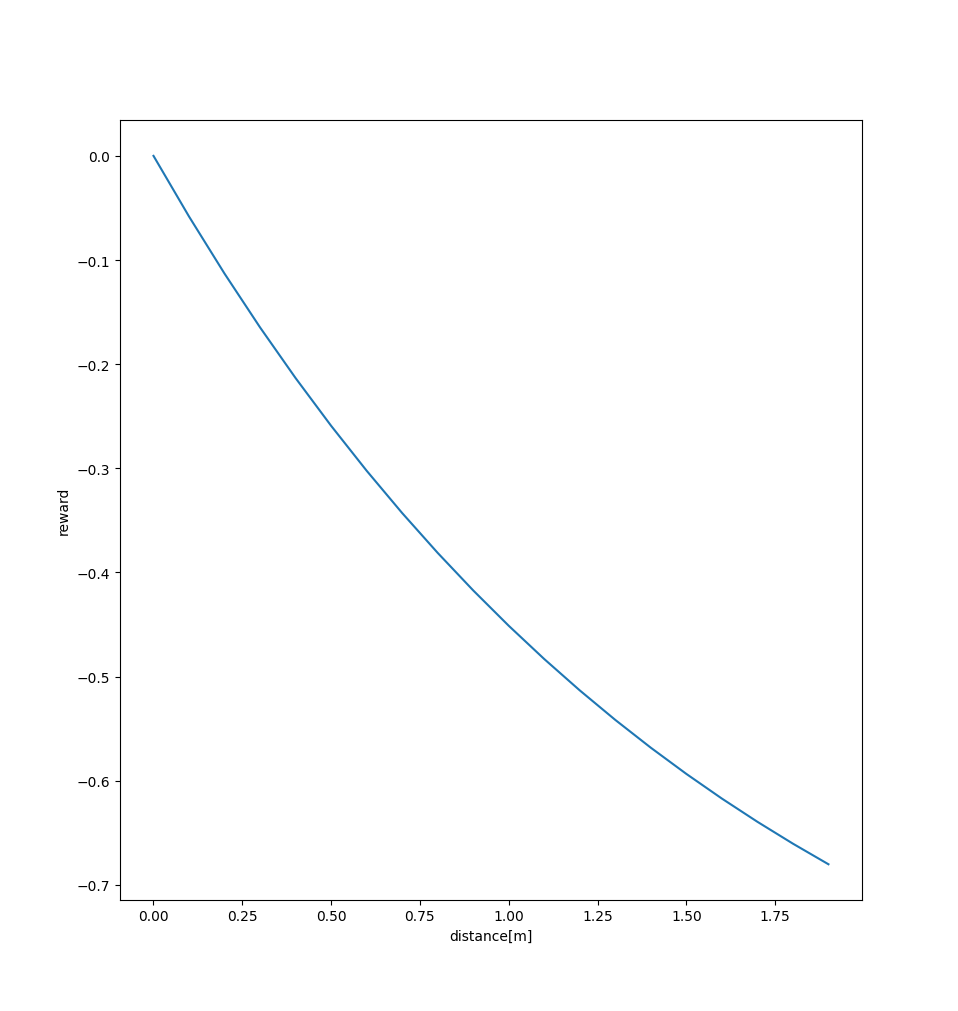
\includegraphics[width= 0.5\linewidth]{figures/reward.png}
	\caption{Visualization of the reward functions over the total distance[m]}
\end{figure}

\subsubsection{Constraints}
\begin{align}
	z_{p_t} \leq z_{min} \land \frac{t}{f} \geq 0.1 \to r_t = e^{-0.6 \cdot |goal - pos|} - 1 -200 \land done
\end{align}

\newpage

\subsubsection{Optimal Rewards}
Based on the modes (\cref{sec:modes}) different optimal rewards (\cref{eq:rew}) can be defined, that are helpful in order to determine how good the learned desicion making is.\\
\newline
\emph{Mode 0} is due to its fixed goal position $g$ rather easy to define:
\begin{align}
R_{opt} &= \sum_{t=0}^{f \cdot episode\_len} r_t \label{eq:oprew}\\
d_0 &= 0.5\\
d_{t+1} &= d_t - |v_{opt}| \cdot \frac{1}{f} \label{eq:dt1}%\\
%r_{t} &= e^{-0.6 \cdot (d_{t+1} )} - 1 \label{eq:rew2}
\end{align}
The distance at start $d_0$ is always 0.5. An optimal decision of the agent corresponds to an optimal velocity vector $v_{opt}$ that minimizes the distance to the goal with the given bounds of the maximum speed at the $\alpha$ of the action processing. The reward (\cref{eq:rew}) can then be used for every control step and summed up to the total optimal reward $R_{opt}$ (\cref{eq:oprew}).\\
\newline
Since \emph{mode 1} does not posess a fixed goal position, only a expected optimal reward $\mathbb{E}(R_{opt})$ can be defined. Therefore, an expected starting distance $\mathbb{E}(d_0)$ has to be used:
\begin{align}
	\mathbb{E}(d_0) &= \sqrt{\mathbb{E}(d_x)^2 + \mathbb{E}(d_y)^2 + \mathbb{E}(d_z)^2} \\
	\mathbb{E}(d_i) &= \int_{b_{min}}^{b_{max}} |i| di \\
	&= 
	\left\{
	\begin{array}{ll}
		 \int_{b_{min}}^{b_{max}} i di & \mbox{if } 0 \leq b_{min} \leq b_{max} \\
		 \int_{b_{min}}^{b_{max}} -i di & \mbox{if } b_{min} \leq b_{max} \leq 0\\
		\int_{b_{min}}^{0} -i di + \int_{0}^{b_{max}} i di  & \mbox{if } b_{min} \leq 0 \leq b_{max}
	\end{array}
	\right. \\
	&=
	\left\{
	\begin{array}{ll}
		\frac{1}{2} \cdot (b_{max}^2 - b_{min}^2) \enspace \enspace \enspace \enspace  & \mbox{if } 0 \leq b_{min} \leq b_{max} \\
		\frac{1}{2} \cdot (b_{min}^2 - b_{max}^2)  & \mbox{if } b_{min} \leq b_{max} \leq 0\\
		\frac{1}{2} \cdot (b_{min}^2 + b_{max}^2) & \mbox{if } b_{min} \leq 0 \leq b_{max}
	\end{array}
	\right.
	\label{eq:expd}
	%\int_{b_{min}}^{0} -i di + \int_{0}^{b_{max}} i di = [-\frac{1}{2}i^2]_{b_{min}}^{0} + [\frac{1}{2}i^2]_0^{b_{max}}\\
	%&= -(- \frac{1}{2} b_{min}^2) + \frac{1}{2} b_{max}^2 = \frac{1}{2} \cdot (b_{min}^2 + b_{max}^2)
\end{align}
The expected distance in each axis $\mathbb{E}(d_i)$ mostly depend on the defined bounds of the goal.\\
\newline
All other modes possess a wind class that trys to disrupt the agent. Since there are random wind fields and the corresponding force is not noramlly distributed, the optimal reward can just estimated downwords. Therefore, the used maximum wind force $W$ is used in order to approximate the maximum of disruptive distance and use it in order to update \cref{eq:dt1}.
\begin{align}
	d_{t+1} &= d_t - | v_{opt} | \cdot \frac{1}{f} + \frac{W}{m} \cdot \frac{1}{f}
\end{align}
\newpage

\subsection{WindSingleAgentPathfollowingAviary Environment Class}


\newpage

%%%%%%%%%%%%%%%%%%%%%%%%%%%%%%%%%%%%%%%%%%%%%
\section{Scripts \& Evaluation Tools} \label{sec:scripts}


%\subsection{TestInstall Script}

\subsection{Learning Script}
\begin{algorithm}
	\caption{Learning Script}
	\label{alg:learn}
	\KwIn{parsed arguments $\xi$}
	 
	 Check the parsed arguments $\xi$ on contradiction and raise ParsingError if needed
	 
	 Create training environment $\epsilon_t$ with the parsed environment args $\lambda \subset \xi$
	 
	 Define the size of the actor and critic policy network
	 
	 \If{parsed load parameter $\iota \in \xi$}{
	 	Load model $\pi$
	 }
	 \Else{
	 	Create model $\pi$
	 }
	 
	 Create evaluation environment $\epsilon_t$ with the parsed environment args $\lambda \subset \xi$
	 
	 Define evaluation callbacks
	 
	 \If{parsed curriculm parameter $\zeta \in \xi$ is parsed as false}{
	 	Learn the model with the parsed amount of time steps
	 }
	 \Else{
	 	Learn the model with the curriculm method (\cref{alg:curri})
	 }
	 
	 Save the model $\pi$ with the parsed preferred name
	 
	 
\end{algorithm}

\newpage

\subsubsection{Exponentiell Curriculm Learning}

\begin{algorithm}
	\caption{Exponentiell Curriculm Learning Algorithm}
	\label{alg:curri}
	\KwIn{total steps $t_{total}$,  set of environment args $\lambda$, model $\pi$, number of parallel environments $\eta$, name, the minimum curriculm step $\gamma$}
	
	Initialize an empty set of curriculm steps $\Gamma$
	
	\Repeat{$t_{total}$ < $\gamma$}{
		\If{last repetition step}{$\Gamma = \Gamma \cup t_{total}$}
		\Else{$\Gamma = \Gamma \cup \gamma$}
		
		$t_{total} = t_{total} - \gamma$
		
		$\gamma = 2^{\gamma}$  
	}
	
	Initialize current radius $r=0$
	
	Get desired radius $r^*$ from $\lambda$
	
	\For{each $\gamma \in \Gamma$}{
		Change radius in $\lambda$ to $r$
		
		Initialize training environment $\epsilon_t$ with $\lambda, \eta$ as parameters
		
		Set the environment of $\pi$ to $\epsilon_t$
		
		Initialize evaluation environment $\epsilon_e$ with $\lambda, \eta$ as parameters
		
		Define evaluation callbacks
		
		Learn the model $\pi$ with an amount of $\gamma$ steps 
		
		Save the model
		
		$r =  \frac{r^*}{|\Gamma| - 1 }$
	}
\end{algorithm}

\newpage

\subsection{Evaluation Script}
\begin{algorithm}
	\caption{Evaluation Script}
	\label{alg:eval}
	\KwIn{parsed arguments $\xi$}
	Check the parsed arguments $\xi$ on contradiction and raise ParsingError if needed
	
	Create evaluation environment $\epsilon_e$ with the parsed environment args $\lambda \subset \xi$
	
	Load the model $\pi$
	
	Instantiate an EvalWriter and evaluate the model $\pi$
	
	\If{parsed gui parameter $\rho \in \xi$}{
		Instantiate a test environement $\epsilon_t$, logger and a pathplotter
		
		Reset environment and safe an observation $\sigma$
		
		Safe current time $t$
		
		\Repeat{done or time is over}{
		Get action $a$ and the observation $\sigma$
		
		Execute a step in the test environment and receive an observation $\sigma$, a reward $r$, a done value and a info
		
		Add current pose $p$ to pathplotter
		
		Log current drone state $s$
		
		Sync simulation time $t_sim$ to the real time $t$}
		Close test environment, show the plotted path and the values.
	}


\end{algorithm}

\newpage

%%%%%%%%%%%%%%%%%%%%%%%%%%%%%%%%%%%%%%%%%%%%%%
\subsection{Evaluation Tools} \label{sec:tools}

\subsubsection{EvalWriter Class}

\newpage

\subsubsection{PathPlotter Class}
